% Adapted from Atanasio Rubio Gil's https://gitlab.com/Groctel/aqademia/-/blob/main/demo/demo_aqademia.tex

\documentclass[10pt, a4paper]{aqademic}

% Language and input encoding

\usepackage[spanish]{babel}

% Document settings

\usepackage[type=CC, modifier=by-nc-sa, version=4.0]{doclicense}
\usepackage{graphicx}
	\graphicspath{{img/}}
\usepackage{multirow}

\author{Daniel Pedrosa Montes - Grupo A2}
\title{Metaheurísticas. Problema de la Mínima Dispersión Diferencial.}

% Document composition

\begin{document}

\AqMaketitle[%
	cover    = identidad_ugr,
    subtitle = Algoritmos Voraz y Búsqueda Local,
    dni      = {{DNI goes here}},
    email    = {{email goes here}},
	url      = https://github.com/moshidev/MH,
    date     = abril del 2022
]

\tableofcontents

\chapter{El Problema de la Mínima Dispersión Diferencial}
    
El Problema de la Mínima Dispersión Diferencial es un problema de optimización combinatoria NP-Completo.\cite{Seminario2MH}

Este se presenta en distintas situaciones como al decidir la localización de instalaciones públicas,
la selección de grupos homogéneos, la identificación de grafos densos/regulares o el reparto equitativo en problemas de
flujo de red.\cite{DUARTE201546}

Intuitivamente estamos ante el Problema de la Mínima Dispersión Diferencial cuando dado un conjunto finito de puntos queremos
seleccionar un subconjunto de estos de forma que todos estén más o menos a la misma distancia unos de otros.

\section{Formulación del Problema}

Podemos describir el problema como
$$\textrm{Minimizar } Max_{i\in M}\{\sum_{j\in M}^{}d_{ij}\}-Min_{i\in M}\{\sum_{j\in M}^{}d_{ij}\} $$
Donde $M$ es un subconjunto de $N$, el conjunto de todos los posibles puntos y donde $d_{ij}$ es la distancia desde dos puntos $i$ y $j$.
$|M| = m$, siendo $m$ el número de elementos a escoger de $N$.

\section{Algoritmos para la resolución aproximada en tiempo polinomial}

La complejidad de este problema nos obliga a utilizar algoritmos que puedan encontrar el óptimo de una forma aproximada en un tiempo de computación razonable.
Entre las técnicas más populares podemos destacar GRASP, Búsqueda Local o métodos basados en Poblaciones.\cite{MDP2010}

Implementaremos, entre otros, algoritmos de tipo Greedy y de Búsqueda Local. Son algoritmos eficientes de por sí, pero para
mejorar la eficiencia de estos será necesario factorizar el cálculo de las soluciones a partir de una solución anterior de forma
que el algoritmo ejecute el número mínimo posible de operaciones al navegar por el espacio de soluciones.
    
\chapter{Arquitectura de la Solución}
    El objetivo principal del software es el de encontrar soluciones al Problema de la Mínima Dispersión Diferencial lo más cercanas
al óptimo posible y de forma que pueda ejecutarse en un tiempo computacional razonable eficientemente posible. Para conseguir esto
implementamos distintas técnicas de búsqueda, en este caso en concreto utilizando técnicas Greedy y de Búsqueda Local.

\section{Filosofía tras la implementación}

Buscando separar mecanismos de políticas y delimitar claramente las responsabilidades entre clases intentamos generalizar en
distintos módulos lógicos. Después de un proceso iterativo descubrimos que los datos, ya sean de la matriz de distancias
entre puntos o de la solución, son independientes a los algoritmos.
Los algoritmos dependen en estos, pero no al contrario. Por tanto los algoritmos dependen en dos módulos:

    1. Un módulo dedicado a ofrecer mecanismos para importar y acceder a los datos y
    
    2. otro módulo para modificar u obtener información sobre una solución.

Esta separación permite ocultar los detalles acerca de la estructura de datos concreta utilizada tanto como para representar
la información de las distancias entre dos puntos como para representar
la solución al algoritmo. Además, salva a la implementación de este de tener en cuenta todas las operaciones necesarias
para calcular la solución de forma factorizada, pudiendo reutilizarse este código en algoritmos futuros y pudiendo adoptar estructuras
de datos más eficientes en un futuro sin tener por ello que cambiar el código concreto del algoritmo.

Así, los algoritmos describen únicamente las políticas sobre los mecanismos de las estructuras de datos en las que dependen.

\begin{figure}[ht]
    \centering
    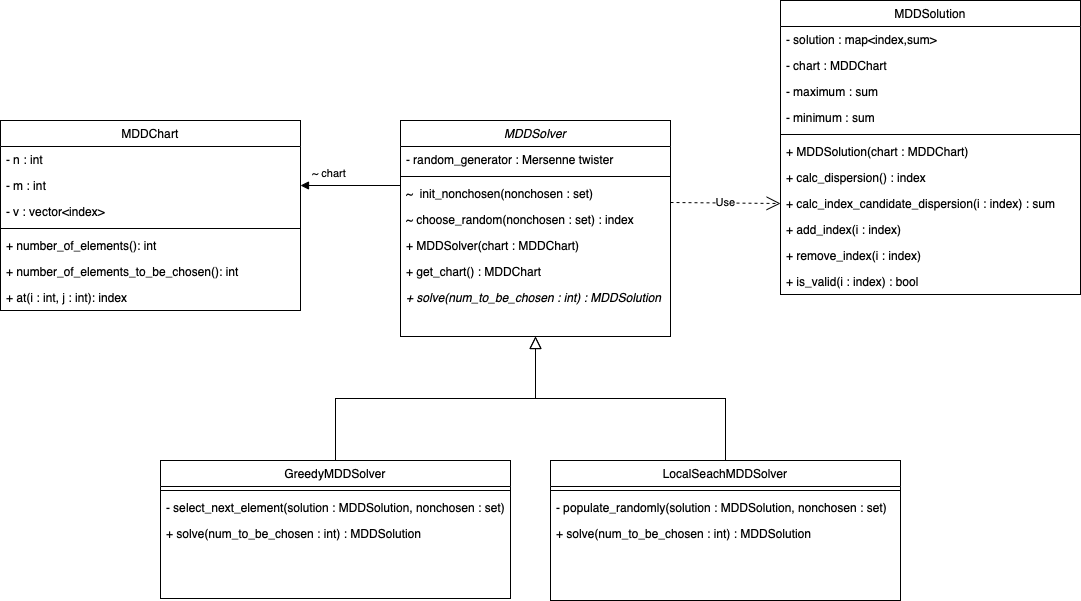
\includegraphics[width=\textwidth]{DiagramaClasesArquitectura.drawio.png}
    \caption{Diagrama de Clases de la solución.}
\end{figure}

\section{Estructuras de datos comunes}

Para representar la matriz que define las distancias entre puntos utilizamos un vector para favorecer la localidad espacial y
temporal de la memoria al realizar un acceso secuencial, como cuando se da el caso cuando necesitamos añadir un punto a una solución.
Gracias a una función constructura podemos leer estos datos de un fichero de texto plano, el cual indica tanto las distancias entre
puntos como el número de puntos existentes en el archivo asi como el número de puntos a seleccionar.

Por otra parte para representar una solución utilizamos un diccionario. Hay alternativas más eficientes, como utilizar un vector binario.
Por ahora esto no nos preocupa, ya que las soluciones se obtienen en un tiempo aceptable aun para instancias grandes del problema y 
al estar abstraidos los mecanismos concretos para actuar sobre la estructura de datos interna concreta que almacena la solución del
algoritmo será fácil de cambiar en un futuro en caso de ser necesario sin afectar por ello a la implementación de los algoritmos. La
interfaz para actuar sobre la solución nos permite añadir y extraer puntos de la solución de la forma más eficiente posible, además
de poder estimar la dispersión de un punto determinado sobre una solución concreta sin tener que añadirlo a la solución en sí. Para
conseguir esto guardamos en el diccionario tanto los puntos escogidos para una solución en concreto como la suma de la distancia desde
el punto al resto de puntos en la solución. En general, estas implementaciones son fruto de unas decisiones de diseño concretas, como la
separación de responsabilidades anteriormente mencionadas, la modificación de un estado únicamente cuando sea necesario, la no pesimización
del código y el cálculo eficiente. Además, minimizamos al máximo la copia y la redundancia de los datos del problema, algoritmo y solución,
ya sea permanente o temporal.

También generalizamos la interfaz de los algoritmos de forma que no sea necesario conocer en tiempo de compilación la implementación
concreta del algoritmo que resuelva el problema.

\section{Aspectos que comparten los distintos algoritmos}

Ambos algoritmos buscan encontrar los puntos pertenecientes al conjunto dado de tal que formen una solución válida y minimicen la dispersión
entre ellos. Por tanto la función objetivo de los algoritmos buscarán encontrar las soluciones tal que $ Disp(Sol^{\prime}) < Disp(Sol) $.

Para tener memoria de los no escogidos en la solución que se devolverá los algoritmos mantienen durante la ejecución del algoritmo un
conjunto de puntos no escogidos que se va actualizando cada vez que se añade, retira o intercambia un punto de la solución.

\section{Añadir y eliminar puntos de la solución. Cálculo de la dispersión de una solución o posible solución}

Como comentamos superficialmente en secciones anteriores la inserción y eliminación de un punto de la solución está implementada de tal
forma que consuma la cantidad mínima de recursos en tiempo, consiguiendo realizar ambas en orden $ \Theta(m) $, siendo $ m $ el 
número de puntos en la solución después de insertar o antes de eliminar.

Para conseguir esto seguimos el algoritmo definido en pseudocódigo en la función \texttt{inserta\_punto\_en\_solucion}, el cual es también bastante parecido
a la función \texttt{elimina\_punto\_de\_solucion}.

\begin{minipage}{\textwidth}
\begin{lstlisting}[mathescape=true,caption={Definición en pseudocódigo de las funciones que permiten añadir y eliminar puntos a una solución.},captionpos=b]
def suma_distancias_desde_un_punto_hasta_los_puntos_de_una_solucion(v, solucion):
    sum = 0
    por cada punto p en solucion:
        sum = sum + distancia(v, p)
    devuelve sum

def inserta_punto_en_solucion(v, solucion):
    si v $ \in $ solucion:
        aborta

    por cada punto p en solucion:
        p.suma_distancias = p.suma_distancias + distancia(v, p)
    
    v.suma_distancias =
        suma_distancias_desde_un_punto_hasta_los_puntos_de_una_solucion(v, solucion)
    solucion.inserta(v)

def elimina_punto_de_solucion(v, solucion):
    si v $ \notin $ solucion:
        aborta
    
    por cada punto p en solucion:
        p.suma_distancias = p.suma_distancias - distancia(v, p)
    
    solucion.elimina(v)
\end{lstlisting}
\end{minipage}

Además, declaramos y definimos una función con nombre \texttt{calcula\_dispersion\_de\_punto\_candidato} para calcular
la dispersión que tendríamos si añadiésemos un determinado punto a la solución.

\begin{minipage}{\textwidth}
\begin{lstlisting}[mathescape=true,caption={Definición de la función que nos permite calcular la dispersión de un punto candidato si perteneciese a una solución.},captionpos=b]
def calcula_dispersion_de_punto_candidato(v, solucion):
    min = $ + \infty $
    max = $ 0 $
    sum_v =
        suma_distancias_desde_un_punto_hasta_los_puntos_de_una_solucion(v, solucion)
    max = $ max $(max, sum_v)
    min = $ min $(min, sum_v)

    por cada punto p en solucion:
        sum_punto_sol = p.suma_distancias + distancia(v, p)
        max = $ max $(max, sum_punto_sol)
        min = $ min $(min, sum_punto_sol)
    
    devuelve max - min
\end{lstlisting}
\end{minipage}

\section{Selección de elementos aleatorios}

Para generar números aleatorios hemos utilizado un generador pseudo-aleatorio de tipo Mersenne Twister, inicializado con una semilla.
Para seleccionar un elemento perteneciente a un conjunto hemos utilizado un generador aleatorio que devuelve valores en una distribución uniforme
el cual utiliza como motor el generador mencionado anteriormente.

\chapter{Resolución del Problema de la Mínima Dispersión Diferencial tomando aproximaciones Greedy y de Búsqueda Local}
    Implementamos dos algoritmos que nos ofrecen siempre que la haya una solución válida, más o menos cercana al óptimo.
En concreto un algoritmo de tipo Greedy y otro de Búsqueda Local, caracterizándose respectivamente por ir cogiendo de entre
los puntos no escogidos los que menos dispersión resultan y por partir de una solución inicial aleatoria e ir buscando de
entre los vecinos el primer mejor que mejora la dispersión de la solución que se mantenga en ese momento hasta haber llegado
a un número determinado de iteraciones o hasta no encontrar vecinos que mejoren la dispersión de la solución.

\section{Aproximación Greedy}

Como hemos mencionado anteriormente la estrategia detrás de nuestra aproximación Greedy es la de ir seleccionando
el punto que minimizaría la dispersión de la solución de entre los no seleccionados parando de añadir puntos a la
solución cuando esta fuese una solución válida. Podemos definir el algoritmo en pseudo-código como sigue:

\begin{minipage}{\textwidth}
\begin{lstlisting}[mathescape=true,caption={Definición del algoritmo Greedy.},captionpos=b]
def selecciona_punto_siguiente(solucion, puntos_no_escogidos):
    elemento_siguiente = puntos_no_escogidos[0]
    dispersion_del_elemento_siguiente = $ + \infty  $
    
    por cada punto p en puntos_no_escogidos:
        dispersion = solucion.calcula_dispersión_de_punto_candidato(p)
        si dispersion < dispersion_del_elemento_siguiente:
            elemento_siguiente = p
            devuelve elemento_siguiente
    
    devuelve elemento_siguiente

def solve(numero_de_puntos_a_elegir, mapa_distancias):
    solucion = new Solucion.asocia(mapa_distancias)
    puntos_no_escogidos = new Set.init(Rango(0, mapa_distancias.numero_de_puntos()))

    primer_punto = escoger_aleatorio(puntos_no_escogidos)
    solucion.inserta_punto_en_solucion(primer_punto)
    puntos_no_escogidos.elimina(primer_punto)
    por cada punto a elegir - 1:
        punto_escogido = selecciona_punto_siguiente(solucion, puntos_no_escogidos)
        solucion.inserta_punto_en_solucion(punto_escogido)
        puntos_no_escogidos.elimina(punto_escogido)
    
    devuelve solucion
\end{lstlisting}
\end{minipage}

Recordemos que la inserción y eliminación de un punto se realiza en tiempo $ \Theta (m) $ en una solución
y en tiempo $ O (\log n) $ en un conjunto. El cálculo de la dispersión de un nodo candidato también se realiza
en tiempo $ \Theta (m) $.

\section{Aproximación por Búsqueda Local del Primer Mejor}

El objetivo de los algoritmos de Búsqueda Local es el de examinar exhaustivamente el espacio de soluciones próximo
a una solución determinada. El criterio de parada suele involucrar un máximo de iteraciones o la imposibilidad de encontrar
soluciones entre los vecinos. Es muy bueno por tanto encontrando óptimos, pero generalmente locales debido a la naturaleza del proceso
de generación de soluciones alternativas, ya que únicamente busca entre los vecinos contiguos. Por sí solos este tipo de
algoritmos veremos que no ofrecen soluciones mucho mejores a soluciones de tipo Greedy, y que al igual que estos la
calidad de la solución vendrá muy determinada por el conjunto inicial, que se escoge aleatoriamente.

\begin{minipage}{\textwidth}
\begin{lstlisting}[mathescape=true,caption={Definición del algoritmo de Búsqueda Local.},captionpos=b]
def primer_mejor_vecino_quitando_punto_de_solucion(punto_a_quitar, solucion, puntos_no_escogidos):
    solucion_sin_punto = solucion
    solucion_sin_punto.elimina_punto_de_solucion(punto_a_quitar)

    mejor_punto = punto_a_quitar
    mejor_dispersion = solucion.calcula_dispersion()

    por cada punto p en puntos_no_escogidos:
        dispersion = solucion_sin_punto.calcula_dispersion_de_punto_candidato(p)
        si dispersion < mejor_dispersion:
            mejor_punto = p
            devuelve mejor_punto
    
    devuelve punto_a_quitar

def solve(numero_de_puntos_a_elegir, mapa_distancias):
    solucion = new Solucion.asocia(mapa_distancias)
    puntos_no_escogidos = new Set.init(Rango(0, mapa_distancias.numero_de_puntos()))
    inicializa_solucion_aleatoriamente(solucion, puntos_no_escogidos, numero_de_puntos_a_elegir)

    dispersion = $ + \infty $
    mejor_dispersion = solucion.calcular_dispersion()

    mientras mejor_dispersion < dispersion y num_iteraciones < 100.000:
        dispersion = mejor_dispersion
        por cada punto p en solucion:
            supuesto_mejor_punto = primer_mejor_vecino_quitando_punto_de_solucion(p, solucion, puntos_no_escogidos)
            si supuesto_mejor_punto es distinto de p:
                puntos_no_escogidos.inserta(p)
                puntos_no_escogidos.elimina(supuesto_mejor_punto)
                solucion.elimina_punto_de_solucion(p)
                solucion.inserta_punto_en_solucion(supuesto_mejor_punto)
                mejor_dispersion = solucion.calcula_dispersion()
\end{lstlisting}
\end{minipage}

En el capítulo segundo podemos ver que los métodos que nos proporciona la estructura de datos que hemos declarado y definido para representar y hacer
operaciones hacen que la solución esté factorizada según se indica en los requisitos de la práctica. 

\subsubsection{Métodos de exploración del entorno y operador de generación de vecino}

Como hemos mencionado anteriormente nuestro algoritmo parte de una primera solución aleatoria y a partir de esta empieza
a comparar esta solución con soluciones que va generando pertenecientes al espacio de búsqueda y cercanas a esta. Sustituye
a la solución elegida con el primer mejor vecino que encuentre.

Podemos ver en la función \texttt{primer\_mejor\_vecino\_quitando\_punto\_de\_solucion} del listado 3.2 el algoritmo
para generar soluciones adyacentes dada una solución, de forma que devuelve la primera mejor solución que encuentre.

Intuitivamente se podría describir como si cogiésemos una solución y le quitásemos un punto que pertenezca a esta.
Una vez hecho esto calculamos la dispersión que tendría una posible solución con cada uno de los puntos pertenecientes
al conjunto de los no escogidos. Si encontramos un punto no seleccionado con mejor dispersión devolvemos la solución
con ese punto, en caso contrario devolvemos la solución original. Cabe destacar que esta descripción es aproximada,
no es lo que se describe exactamente en el algoritmo.

\begin{figure}[ht]
    \centering
    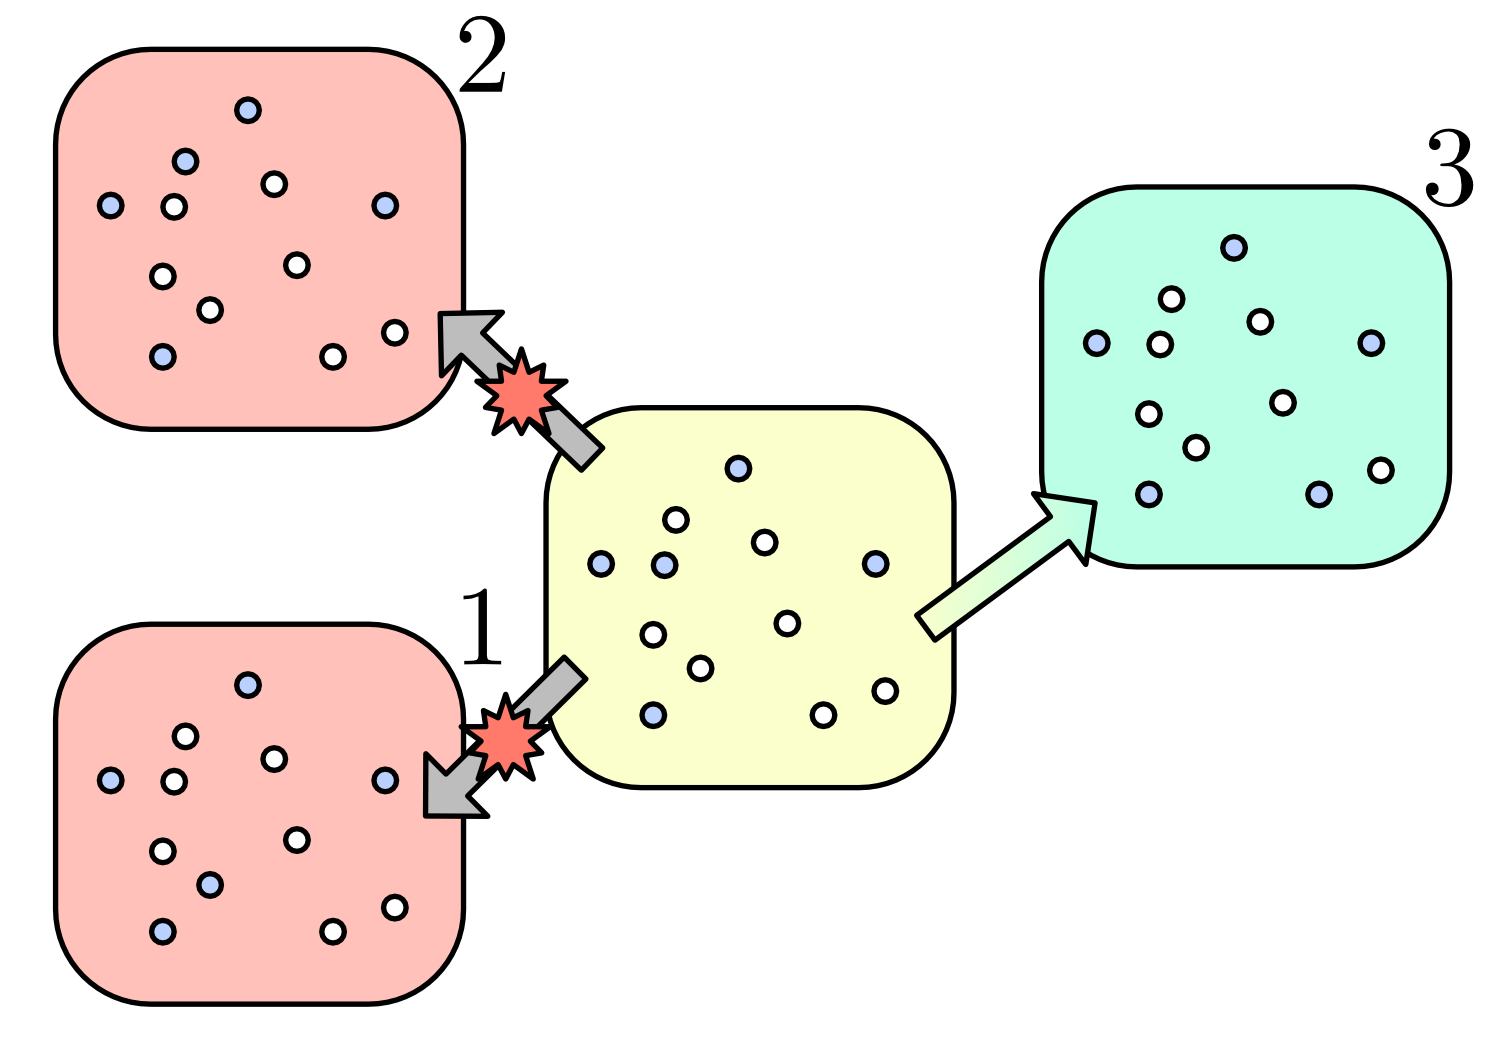
\includegraphics[height=7.5cm,keepaspectratio]{busqueda_local_exploracion.png}
    \caption{Generación y selección de vecinos en el algoritmo de Búsqueda Local Primero el Mejor. Las soluciones se generan en el orden 1, 2, 3. En el momento en el que encuentra una solución mejor, la tercera en este caso, la devuelve.}
\end{figure}

\subsubsection{Generación de soluciones aleatorias}

En el listado 3.2 hacemos referencia a una función llamada \texttt{inicializa\_solucion\_aleatoriamente}.
La definimos en el siguiente listado.

\begin{minipage}{\textwidth}
\begin{lstlisting}[mathescape=true,caption={Definición de la función \texttt{inicializa\_solucion\_aleatoriamente} para generar una solución consistente en elementos aleatorios.},captionpos=b]
def inicializa_solucion_aleatoriamente(solucion, puntos_no_escogidos, numero_de_puntos_a_elegir):
    por cada uno de los puntos que tenemos que elegir:
        punto_elegido = escoge_aleatorio(puntos_no_escogidos)
        puntos_no_escogidos.elimina(punto_elegido)
        solucion.inserta_punto_en_solucion(punto_elegido)
\end{lstlisting}
\end{minipage}

\bibliographystyle{plain}
\bibliography{references}

\end{document}
